\documentclass[a4paper,12pt]{article}
\usepackage[utf8]{inputenc}
\setlength{\marginparwidth}{2cm}
\usepackage{todonotes}
\usepackage[russian]{babel}
\usepackage{graphicx}
\usepackage{amsmath, amssymb}
\usepackage{hyperref}
\usepackage{float}
\usepackage{listings}
\usepackage{caption}
\usepackage{geometry}
\usepackage{xcolor}
\geometry{left=2cm,right=2cm,top=2cm,bottom=2cm}
\hypersetup{pdfborder=0 0 0}
\headsep=8mm
\footskip=20mm
\hypersetup{pdfstartview=FitH, linkcolor=linkcolor, urlcolor=urlcolor, colorlinks=true}

\definecolor{strings}{rgb}{0,0.6,0}
\definecolor{comments}{rgb}{0,0.3,0}
\definecolor{numbers}{rgb}{0.5,0.5,0.5}
\definecolor{keywords}{rgb}{0.09,0.61,0.95}
\definecolor{background}{rgb}{0.97,0.97,0.97}

\lstdefinestyle{codestyle}{
    backgroundcolor=\color{background},
    commentstyle=\color{comments},
    keywordstyle=\color{keywords},
    stringstyle=\color{strings},
    numberstyle=\tiny\color{numbers},
    basicstyle=\ttfamily\scriptsize,
    breakatwhitespace=false,
    breaklines=true,
    captionpos=b,
    inputencoding=utf8,
    keepspaces=false,
    numbers=left,
    numbersep=5pt,
    showspaces=false,
    showstringspaces=false,
    showtabs=false,
    tabsize=2,
    extendedchars=true
}

\lstset{style=codestyle}

\begin{document}    

% Титульный лист
\begin{titlepage}
    \centering
    {\large Федеральное государственное автономное образовательное учреждение\par}
    {\large высшего образования\par}
    {\bfseries САНКТ-ПЕТЕРБУРГСКИЙ НАЦИОНАЛЬНЫЙ ИССЛЕДОВАТЕЛЬСКИЙ УНИВЕРСИТЕТ ИТМО\par}
    {\bfseries Факультет систем управления и робототехники\par}
    \vfill
    {\Large \bfseries Лабораторная работа №3\par}
    {\Large \bfseries Фильтрация и выделение контуров\par}
    \vfill
    
    \begin{flushright}
        Студенты: Бахтаиров Р.А.,\\ Сайфуллин Д.Р. \\
        Поток: Тех.Зр R23 1.1 \\
        Преподаватель: Шаветов С.В.
    \end{flushright}
    \vfill
    Санкт-Петербург, 2025 г.
\end{titlepage}

% Оглавление
\tableofcontents
\newpage

% Введение
\section{Цель работы}
В этой работе мы ознакомимся с основными способами фильтрации изображений от шумов, изучим алгоритмы выделения контуров.

\section{Изображение, с которым будем работать}
\begin{figure}[H]
    \centering
    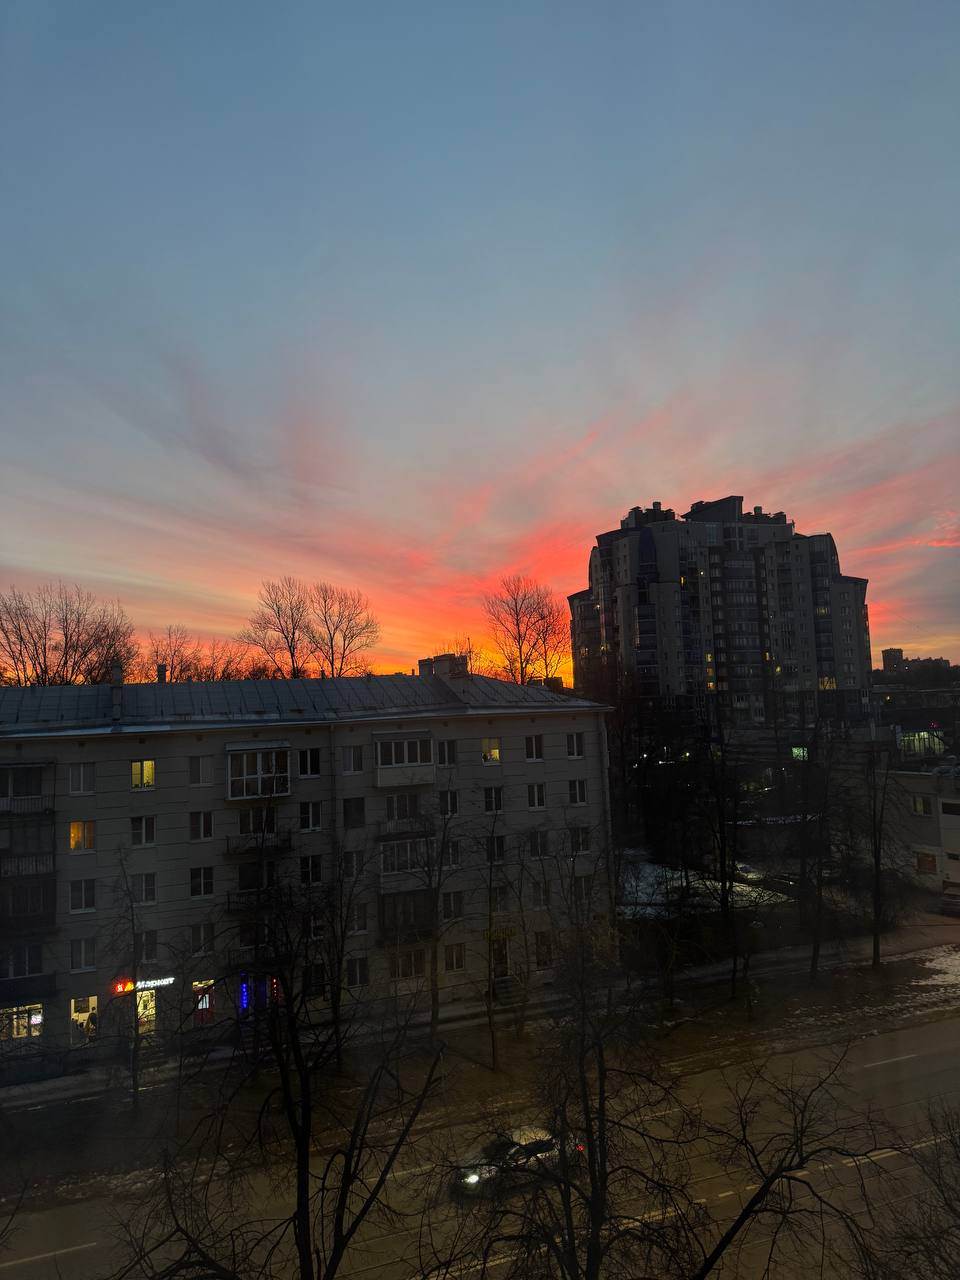
\includegraphics[width=0.7\textwidth]{images/my_img.png}
\end{figure}

\section{Типы шумов}    
В этом разделе описаны типы шумов, используемые в лабораторной работе.
\begin{enumerate}
    \item  Импульсный шум
    \item  Мультипликативный шум        
    \item  Гауссов (нормальный) шум     
    \item  Шум квантования
\end{enumerate}
Рассмотрим как выглядят эти шумы на изображении при разных входных параметрах.
\subsection{Импульсный шум}
Этот вид шума (также известный как "соль-перец") шум характеризуется появлением случайных ярких (белых) или темных (черных) точек в изображении. Его можно смоделировать следующим образом:
\begin{equation*}
    I_{\text{noisy}}(x,y) = 
    \begin{cases}
    I(x,y), & \text{с вероятностью } 1-p,\\
    255, & \text{с вероятностью } p.
    \end{cases}
    \label{eq:impulse}
\end{equation*}
Применим данный вид шума на наше изображение, с помощью функции $imnoise()$, чтобы увидеть, как он влияет на его внешний вид.
\begin{figure}[H]
    \centering 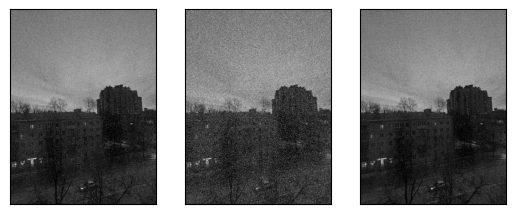
\includegraphics[width=0.9\textwidth]{results/sap_v.png}
    \caption{Наложение импульсного шума на изображение (стандартные параметры, $p=0.2$ и $s=0.5$, $p=0.05$ и $s=0.3$)}
\end{figure}
\noindent
При небольшом значении \(p=0.05\) шум «соль-перец» появляется редко. При повышении \(p\) до \(0.2\) количество шумовых точек значительно увеличивается, в результате чего изображение выглядит значительно более «засорённым». При уменьшении \(s\) до \(0.3\), несмотря на то, что доля шумовых пикселей остаётся \(p=0.05\), их яркостное отклонение становится меньше, и шум воспринимается мягче.

\subsection{Мультипликативный шум}
При данном типе шума интенсивность каждого пикселя изменяется пропорционально своей величине. Такой шум часто моделируется как:
\begin{equation*}
    I_{\text{noisy}}(x,y) = I(x,y) \cdot \eta(x,y),
\end{equation*}
где \(\eta(x,y)\) — случайная величина, не зависящая от сигнала.
Аналогично применим метод на наше изображение:
\begin{figure}[H]
    \centering 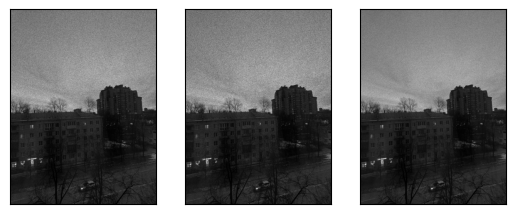
\includegraphics[width=0.9\textwidth]{results/speckle_v.png}
    \caption{Наложение мультипликативного шума на изображение (стандартное отклонение, при $var=0.07$, при $var=0.02$)}
\end{figure}
\noindent
При мультипликативном шуме отклонения пикселей зависят от исходной яркости: более тёмные участки затрагиваются слабее, а более светлые — заметнее. При большем значении \(\text{var} = 0.07\) шумовые искажения оказываются ярче выраженными, особенно в относительно светлых областях, что делает общее качество изображения заметно хуже. При уменьшении \(\text{var} = 0.02\) разброс интенсивностей уменьшается, и искажения выглядят менее агрессивно.

\subsection{Гауссов шум}
Это наиболее распространённый тип шума, возникающий из-за случайных отклонений в системе. Гауссов шум характеризуется нормальным распределением с нулевым средним значением и дисперсией \(\sigma^2\):
\begin{equation*}
    I_{\text{noisy}}(x,y) = I(x,y) + n(x,y), \quad n(x,y) \sim \mathcal{N}(0,\sigma^2).
\end{equation*}
Применим данный вид шума на наше изображение, с помощью функции $imnoise()$, чтобы увидеть, как он влияет на его внешний вид.
\begin{figure}[H]
    \centering 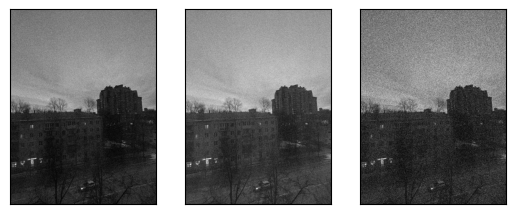
\includegraphics[width=0.9\textwidth]{results/gaussian_v.png}
    \caption{Наложение шума гаусса на изображение (стандартные параметры, $mean=0.1$ и $var=0.1$, $mean=0.0$ и $var=0.05$)}
\end{figure}
\noindent
При добавлении гауссова шума с ненулевым средним изображение слегка осветляется, так как шумовое смещение сдвигает яркость в сторону более светлых значений. Увеличение дисперсии заметно усиливает «зернистость» и яркость по всей площади кадра, делая шум более выраженным. При mean $=0.0$ шум распределён симметрично относительно исходных значений яркости, и изменения воспринимаются в основном как равномерные случайные искажения без общей смены тона.

\subsection{Шум квантования}
Возникает при дискретизации и кодировании изображения, когда непрерывные значения интенсивности преобразуются в конечное число уровней. Ошибка квантования определяется разностью между истинным значением и округленным:
\begin{equation}
    I_{\text{noisy}}(x,y) = Q(I(x,y)) = I(x,y) + \epsilon(x,y),
    \label{eq:quantization}
\end{equation}
где \(\epsilon(x,y)\) --- ошибка квантования, которая обычно принимается равномерно распределённой в диапазоне \([-\Delta/2, \Delta/2]\), \(\Delta\) --- шаг квантования.
Применим данный вид шума на наше изображение:
\begin{figure}[H]
    \centering 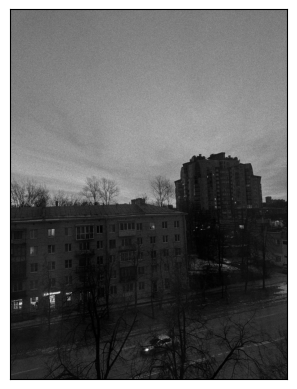
\includegraphics[width=0.3\textwidth]{results/pois.png}
    \caption{Наложение шума квантования на изображение}
\end{figure}

Соберем по одному каждый вид шума в один массив для дальнейшей работы.
\begin{figure}[H]
    \begin{minipage}{0.49\textwidth}
        \centering 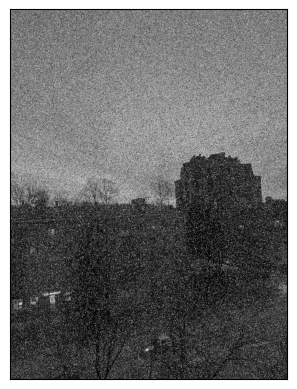
\includegraphics[width=\textwidth]{results/sap.png}
        \caption{Импульсный шум}
    \end{minipage}\hfill
    \begin{minipage}{0.49\textwidth}
        \centering 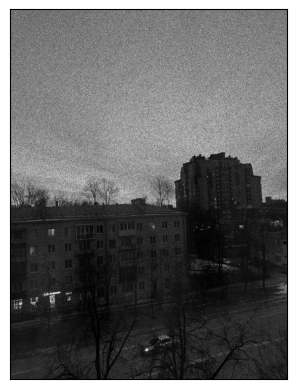
\includegraphics[width=\textwidth]{results/speckle.png}
        \caption{Мультипликативный шум}
    \end{minipage}
\end{figure}
\begin{figure}[H]
    \begin{minipage}{0.49\textwidth}
        \centering 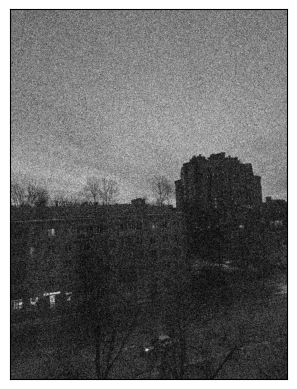
\includegraphics[width=\textwidth]{results/gaus.png}
        \caption{Гауссов шум}
    \end{minipage}\hfill
    \begin{minipage}{0.49\textwidth}
        \centering 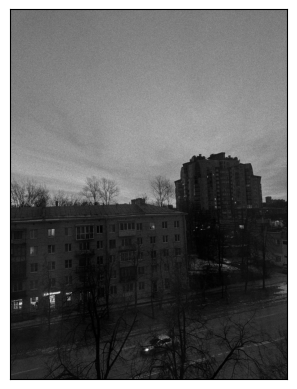
\includegraphics[width=\textwidth]{results/pois.png}
        \caption{Шум квантования}
    \end{minipage}
\end{figure}

\section{Низкочастотные фильтры}
Низкочастотные фильтры предназначены для подавления высокочастотных составляющих изображения (шумов, резких перепадов яркости), сохраняя при этом основные крупные детали. Ниже рассмотрены основные виды таких фильтров.

\subsection{Арифметический усредняющий фильтр}
Арифметический усредняющий фильтр (Arithmetic Mean Filter) вычисляет среднее арифметическое значений интенсивностей пикселей внутри окна размером \(m \times n\):
\begin{equation}
I_{\text{out}}(x,y) \;=\; \frac{1}{mn} \sum_{u=0}^{m-1} \sum_{v=0}^{n-1} I(x+u,\,y+v).
\end{equation}
\begin{figure}[H]
    \begin{minipage}{0.49\textwidth}
        \centering 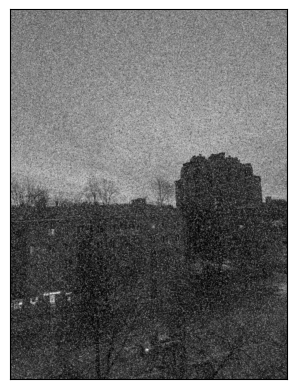
\includegraphics[width=\textwidth]{results/lpf_sap_1.png}
        \caption{Импульсный шум с применением арифметический фильтр}
    \end{minipage}\hfill
    \begin{minipage}{0.49\textwidth}
        \centering 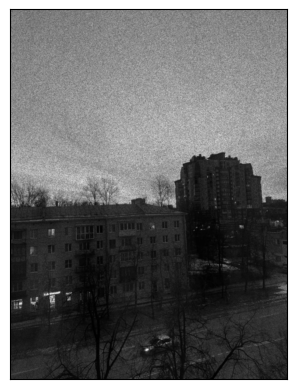
\includegraphics[width=\textwidth]{results/lpf_speckle_1.png}
        \caption{Мультипликативный шум с применением арифметический фильтр}
    \end{minipage}
\end{figure}
\begin{figure}[H]
    \begin{minipage}{0.49\textwidth}
        \centering 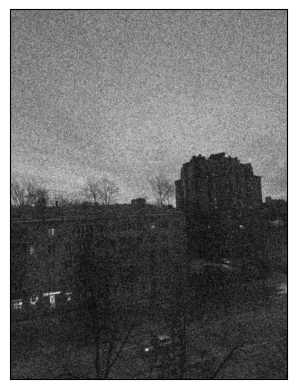
\includegraphics[width=\textwidth]{results/lpf_gaus_1.png}
        \caption{Гауссов шум с применением арифметический фильтр}
    \end{minipage}\hfill
    \begin{minipage}{0.49\textwidth}
        \centering 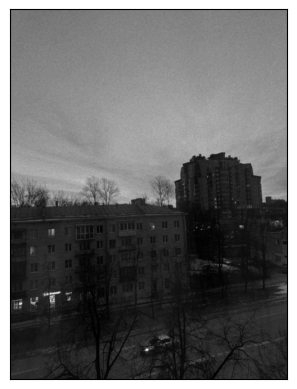
\includegraphics[width=\textwidth]{results/lpf_pois_1.png}
        \caption{Шум квантования с применением арифметический фильтр}
    \end{minipage}
\end{figure}
Он эффективно снижает гауссов и равномерный шум, но может «размывать» резкие границы объектов.

\subsection{Геометрический усредняющий фильтр}
Геометрический усредняющий фильтр (Geometric Mean Filter) вместо суммы использует произведение:
\begin{equation}
I_{\text{out}}(x,y) \;=\;
\left(\,
\prod_{u=0}^{m-1} \prod_{v=0}^{n-1} I(x+u,\,y+v)
\right)^{\tfrac{1}{mn}}.
\end{equation}
\begin{equation}
I_{\text{out}}(x,y) \;=\; \frac{1}{mn} \sum_{u=0}^{m-1} \sum_{v=0}^{n-1} I(x+u,\,y+v).
\end{equation}
\begin{figure}[H]
    \begin{minipage}{0.49\textwidth}
        \centering 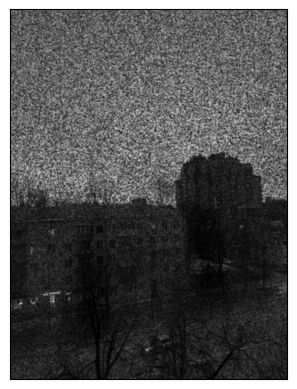
\includegraphics[width=\textwidth]{results/lpf_sap_2.png}
        \caption{Импульсный шум с применением геометрического фильтр}
    \end{minipage}\hfill
    \begin{minipage}{0.49\textwidth}
        \centering 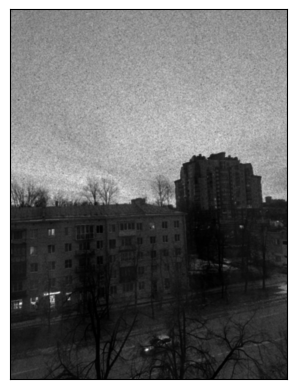
\includegraphics[width=\textwidth]{results/lpf_speckle_2.png}
        \caption{Мультипликативный шум с применением геометрического фильтр}
    \end{minipage}
\end{figure}
\begin{figure}[H]
    \begin{minipage}{0.49\textwidth}
        \centering 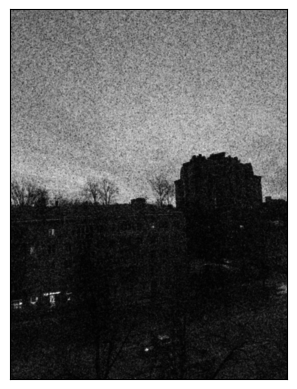
\includegraphics[width=\textwidth]{results/lpf_gaus_2.png}
        \caption{Гауссов шум с применением геометрического фильтр}
    \end{minipage}\hfill
    \begin{minipage}{0.49\textwidth}
        \centering 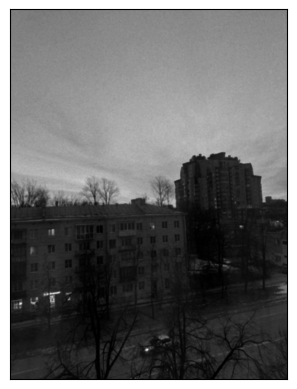
\includegraphics[width=\textwidth]{results/lpf_pois_2.png}
        \caption{Шум квантования с применением геометрического фильтр}
    \end{minipage}
\end{figure}
\noindent
Подобный подход помогает лучше подавлять крупные выбросы (яркие шумовые пиксели), но при этом чувствителен к нулевым или очень малым значениям интенсивности.

\subsection{Гармонический усредняющий фильтр}
Гармонический усредняющий фильтр (Harmonic Mean Filter) определяется формулой:
\begin{equation}
I_{\text{out}}(x,y) \;=\;
\frac{mn}{
\displaystyle \sum_{u=0}^{m-1}\sum_{v=0}^{n-1}
\frac{1}{I(x+u,\,y+v)}
}.
\end{equation}
\begin{figure}[H]
    \begin{minipage}{0.49\textwidth}
        \centering 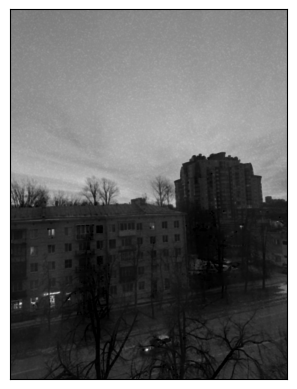
\includegraphics[width=\textwidth]{results/lpf_sap_3.png}
        \caption{Импульсный шум с применением гармонического фильтр}
    \end{minipage}\hfill
    \begin{minipage}{0.49\textwidth}
        \centering 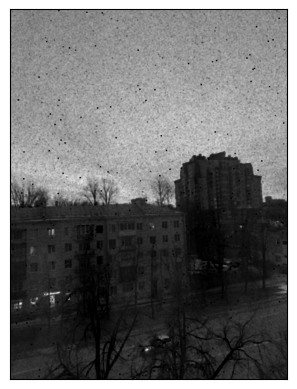
\includegraphics[width=\textwidth]{results/lpf_speckle_3.png}
        \caption{Мультипликативный шум с применением гармонического фильтр}
    \end{minipage}
\end{figure}
\begin{figure}[H]
    \begin{minipage}{0.49\textwidth}
        \centering 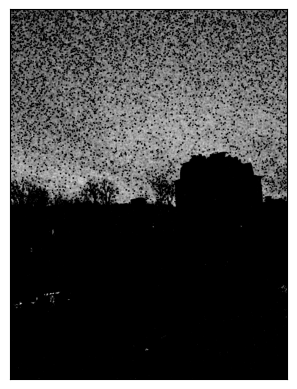
\includegraphics[width=\textwidth]{results/lpf_gaus_3.png}
        \caption{Гауссов шум с применением гармонического фильтр}
    \end{minipage}\hfill
    \begin{minipage}{0.49\textwidth}
        \centering 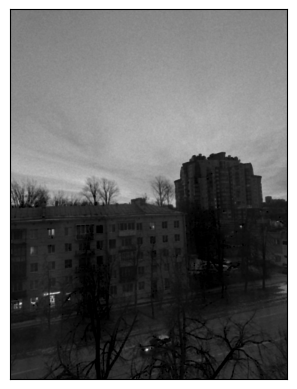
\includegraphics[width=\textwidth]{results/lpf_pois_3.png}
        \caption{Шум квантования с применением гармонического фильтр}
    \end{minipage}
\end{figure}
\noindent
Данный фильтр хорошо подавляет импульсный шум с яркими точками, однако чувствителен к нулевым значениям интенсивности.

\subsection{Контргармонический усредняющий фильтр}
Контргармонический усредняющий фильтр (Counterharmonic Mean Filter) обобщает гармоническое усреднение с дополнительным параметром \(Q\):
\begin{equation}
I_{\text{out}}(x,y) \;=\;
\frac{\displaystyle \sum_{u,v} \bigl(I(x+u,\,y+v)\bigr)^{\,Q+1}}
{\displaystyle \sum_{u,v} \bigl(I(x+u,\,y+v)\bigr)^{\,Q}}.
\end{equation}
В отчете представлены результаты работы фильтра при оптимальных значениях \(Q\) для различных типов шумов.
\begin{figure}[H]
    \begin{minipage}{0.49\textwidth}
        \centering 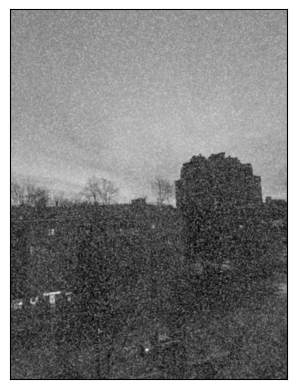
\includegraphics[width=\textwidth]{results/lpf_sap_4.png}
        \caption{Импульсный шум с применением контргармонического фильтр (Q=0.1)}
    \end{minipage}\hfill
    \begin{minipage}{0.49\textwidth}
        \centering 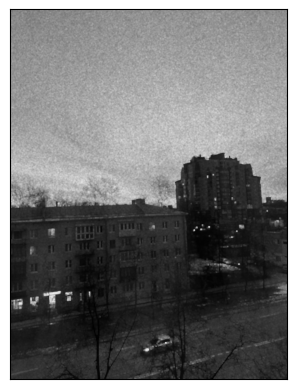
\includegraphics[width=\textwidth]{results/lpf_speckle_4.png}
        \caption{Мультипликативный шум с применением контргармонического фильтр (Q=5.0)}
    \end{minipage}
\end{figure}
\begin{figure}[H]
    \begin{minipage}{0.49\textwidth}
        \centering 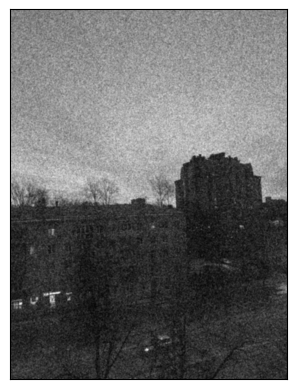
\includegraphics[width=\textwidth]{results/lpf_gaus_4.png}
        \caption{Гауссов шум с применением контргармонического фильтр (Q=2.0)}
    \end{minipage}\hfill
    \begin{minipage}{0.49\textwidth}
        \centering 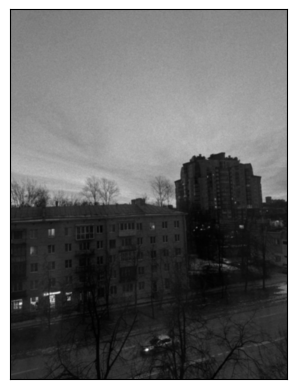
\includegraphics[width=\textwidth]{results/lpf_pois_4.png}
        \caption{Шум квантования с применением контргармонического фильтр (Q=0.1)}
    \end{minipage}
\end{figure}
\noindent
При \(Q>1\) фильтр лучше подавляет гауссов и мультипликативный шум, при \(Q<1\) --- эффективнее справляется с импульсным шумом.

\subsection{Фильтр Гаусса}
Фильтр Гаусса (Gaussian Filter) вычисляет взвешенное среднее пикселей в окрестности, где веса определяются гауссовым распределением:
\begin{equation}
I_{\text{out}}(x,y) \;=\;
\sum_{u=-k}^{k} \sum_{v=-k}^{k} I(x+u,\,y+v)\;
\frac{1}{2\pi\sigma^2}
\exp\!\Bigl(-\frac{u^2 + v^2}{2\sigma^2}\Bigr),
\end{equation}
где \(\sigma\) --- параметр, определяющий степень сглаживания, а \(2k+1\) --- размер окна фильтра. 
\begin{figure}[H]
    \begin{minipage}{0.49\textwidth}
        \centering 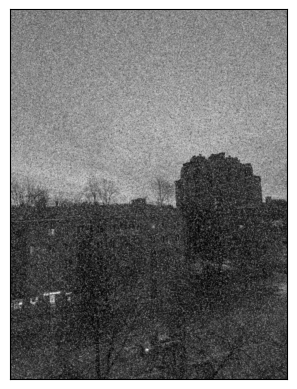
\includegraphics[width=\textwidth]{results/lpf_sap_5.png}
        \caption{Импульсный шум с применением фильтра Гаусса}
    \end{minipage}\hfill
    \begin{minipage}{0.49\textwidth}
        \centering 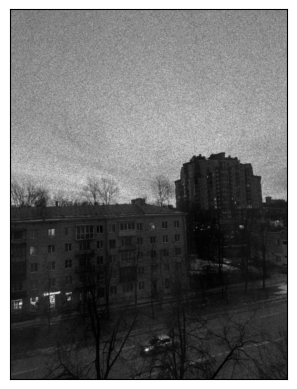
\includegraphics[width=\textwidth]{results/lpf_speckle_5.png}
        \caption{Мультипликативный шум с применением фильтра Гаусса}
    \end{minipage}
\end{figure}
\begin{figure}[H]
    \begin{minipage}{0.49\textwidth}
        \centering 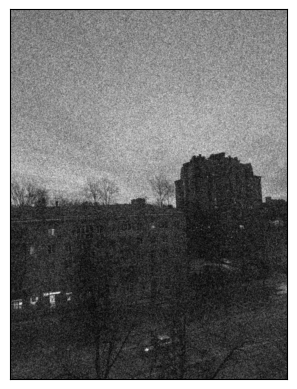
\includegraphics[width=\textwidth]{results/lpf_gaus_5.png}
        \caption{Гауссов шум с применением фильтра Гаусса}
    \end{minipage}\hfill
    \begin{minipage}{0.49\textwidth}
        \centering 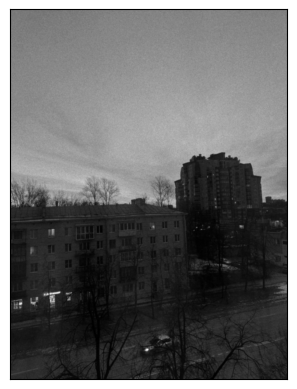
\includegraphics[width=\textwidth]{results/lpf_pois_5.png}
        \caption{Шум квантования с применением фильтра Гаусса}
    \end{minipage}
\end{figure}
\noindent
На различных зашумлённых изображениях лучше всего результат получается при гауссовом шуме. Поскольку гауссов шум имеет распределение, аналогичное форме ядра фильтра, его подавление оказывается наиболее эффективным. При других типах шума Гауссов фильтр также сглаживает искажения, однако может оставлять характерные артефакты или недостаточно подавлять «точечные» выбросы.

\section{Нелинейная фильтраци}
Нелинейные фильтры позволяют учитывать не только локальное усреднение, но и ранговые отношения пикселей в окрестности. Они особенно эффективны для подавления импульсного шума и сохранения резких границ объектов.

\subsection{Медианная фильтрация}
Медианный фильтр заменяет значение пикселя на медиану его локальной окрестности. Пусть \(\Omega_{(x,y)}\) --- множество интенсивностей пикселей в окрестности \((x,y)\), тогда медиана определяется как элемент, делящий упорядоченный список значений на две равные части:
\[
I_{\text{out}}(x,y) = \mathrm{median}\bigl(\Omega_{(x,y)}\bigr).
\]
        \begin{figure}[H]
            \begin{minipage}{0.49\textwidth}
                \centering 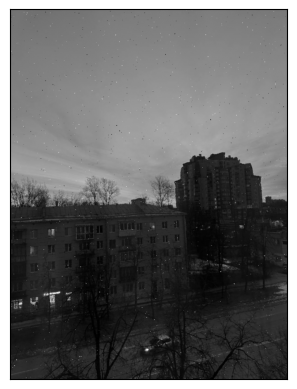
\includegraphics[width=\textwidth]{results/nlf_sap_1.png}
                \caption{Импульсный шум с применением медианного фильтра}
            \end{minipage}\hfill
            \begin{minipage}{0.49\textwidth}
                \centering 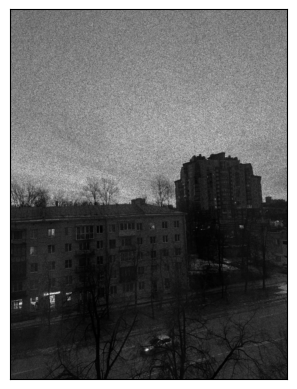
\includegraphics[width=\textwidth]{results/nlf_speckle_1.png}
                \caption{Мультипликативный шум с применением медианного фильтра}
            \end{minipage}
        \end{figure}
        \begin{figure}[H]
            \begin{minipage}{0.49\textwidth}
                \centering 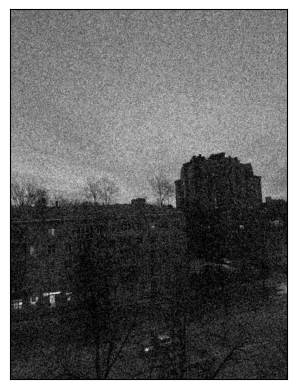
\includegraphics[width=\textwidth]{results/nlf_gaus_1.png}
                \caption{Гауссов шум с применением медианного фильтра}
            \end{minipage}\hfill
            \begin{minipage}{0.49\textwidth}
                \centering 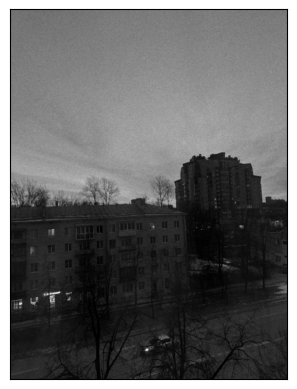
\includegraphics[width=\textwidth]{results/nlf_pois_1.png}
                \caption{Шум квантования с применением медианного фильтра}
            \end{minipage}
        \end{figure}
        \noindent
Такой подход хорошо подавляет «соль-перец» шум, сохраняя при этом относительно резкие границы.

\subsection{Взвешенная медианная фильтрация}
Взвешенный медианный фильтр (Weighted Median Filter) --- обобщение медианной фильтрации, при котором каждому пикселю в окрестности \((x,y)\) приписывается вес \(w_{ij}\). Фактически, пиксель \((i,j)\) повторяется \(w_{ij}\) раз в выборке перед поиском медианы. Это даёт возможность учесть пространственную структуру или иные факторы, повышая или понижая вклад отдельных элементов окрестности.
\begin{figure}[H]
    \begin{minipage}{0.49\textwidth}
        \centering 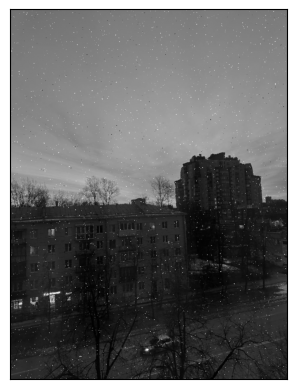
\includegraphics[width=\textwidth]{results/nlf_sap_2.png}
        \caption{Импульсный шум с применением взвешенного медианного фильтра}
    \end{minipage}\hfill
    \begin{minipage}{0.49\textwidth}
        \centering 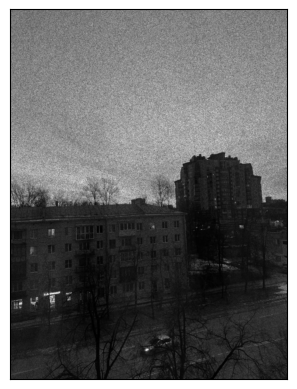
\includegraphics[width=\textwidth]{results/nlf_speckle_2.png}
        \caption{Мультипликативный шум с применением взвешенного медианного фильтра}
    \end{minipage}
\end{figure}
\begin{figure}[H]
    \begin{minipage}{0.49\textwidth}
        \centering 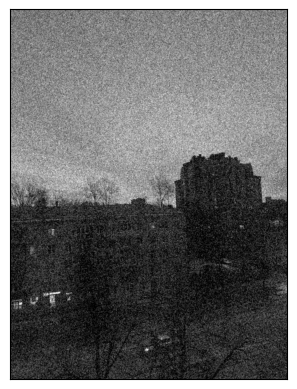
\includegraphics[width=\textwidth]{results/nlf_gaus_2.png}
        \caption{Гауссов шум с применением взвешенного медианного фильтра}
    \end{minipage}\hfill
    \begin{minipage}{0.49\textwidth}
        \centering 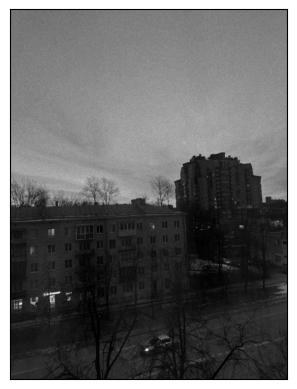
\includegraphics[width=\textwidth]{results/nlf_pois_2.png}
        \caption{Шум квантования с применением взвешенного медианного фильтра}
    \end{minipage}
\end{figure}

\subsection{Адаптивная медианная фильтрация}
Адаптивный медианный фильтр (Adaptive Median Filter) динамически изменяет размер окна при обнаружении сильных выбросов или недостаточной статистики в текущей окрестности:
\begin{enumerate}
    \item Начинаем с окна минимального размера (обычно \(3\times 3\)).
    \item Вычисляем медиану, минимальное и максимальное значение в окрестности.
    \item Если медиана лежит между минимумом и максимумом, переходим к проверке исходного пикселя: если $I(x,y)$ также лежит между минимумом и максимумом, оставляем его, иначе берём медиану.
    \item Если условие не выполняется, увеличиваем размер окна (например, до \(5\times 5\)) и повторяем, пока не достигнем максимального размера.
\end{enumerate}
\begin{figure}[H]
    \begin{minipage}{0.49\textwidth}
        \centering 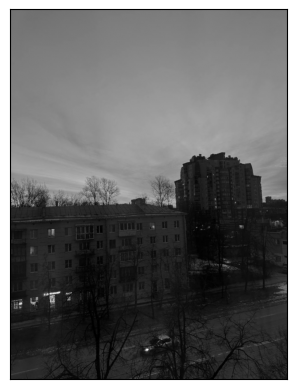
\includegraphics[width=\textwidth]{results/nlf_sap_5.png}
        \caption{Импульсный шум с применением адаптивного медианного фильтра}
    \end{minipage}\hfill
    \begin{minipage}{0.49\textwidth}
        \centering 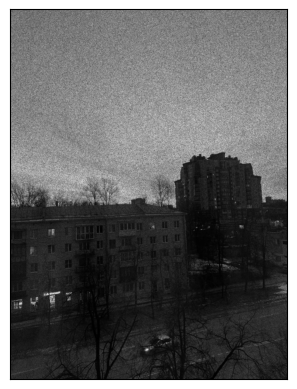
\includegraphics[width=\textwidth]{results/nlf_speckle_5.png}
        \caption{Мультипликативный шум с применением адаптивного медианного фильтра}
    \end{minipage}
\end{figure}
\begin{figure}[H]
    \begin{minipage}{0.49\textwidth}
        \centering 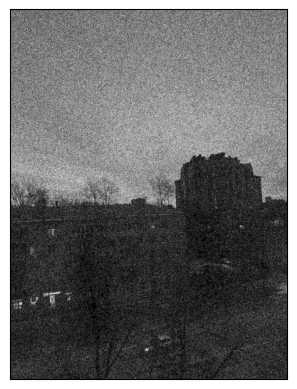
\includegraphics[width=\textwidth]{results/nlf_gaus_5.png}
        \caption{Гауссов шум с применением адаптивного медианного фильтра}
    \end{minipage}\hfill
    \begin{minipage}{0.49\textwidth}
        \centering 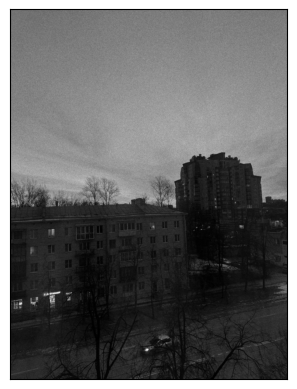
\includegraphics[width=\textwidth]{results/nlf_pois_5.png}
        \caption{Шум квантования с применением адаптивного медианного фильтра}
    \end{minipage}
\end{figure}
\noindent
Данный метод эффективно подавляет импульсный шум, не размывая излишне детали.

\subsection{Ранговая фильтрация}
Ранговый фильтр (Rank Filter) сортирует значения интенсивностей в локальном окне и выбирает элемент с определённым рангом \(r\). Для окна из \(m\times n\) пикселей все значения записываются в отсортированный массив, и фильтр возвращает \(\mathrm{val}[r]\). Частными случаями являются:
\begin{itemize}
    \item \(\mathrm{rank}=0\) --- минимальный фильтр (Min Filter),
    \item \(\mathrm{rank}=mn-1\) --- максимальный фильтр (Max Filter),
\end{itemize}
Взглянем на изображения с минимальным параметром:
\begin{figure}[H]
    \begin{minipage}{0.49\textwidth}
        \centering 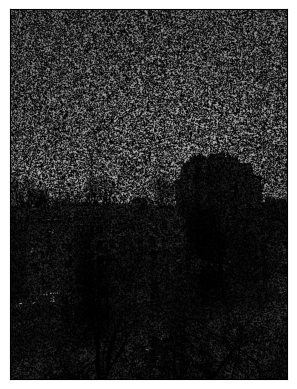
\includegraphics[width=\textwidth]{results/nlf_sap_3.png}
        \caption{Импульсный шум с применением рангового фильтра}
    \end{minipage}\hfill
    \begin{minipage}{0.49\textwidth}
        \centering 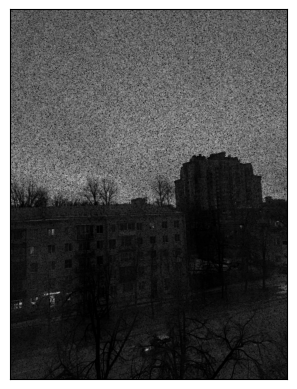
\includegraphics[width=\textwidth]{results/nlf_speckle_3.png}
        \caption{Мультипликативный шум с применением рангового фильтра}
    \end{minipage}
\end{figure}
\begin{figure}[H]
    \begin{minipage}{0.49\textwidth}
        \centering 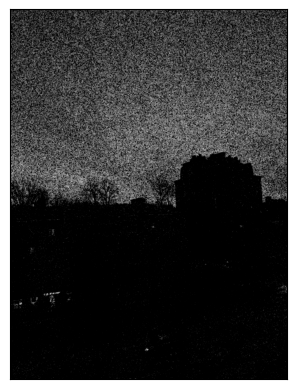
\includegraphics[width=\textwidth]{results/nlf_gaus_3.png}
        \caption{Гауссов шум с применением рангового фильтра}
    \end{minipage}\hfill
    \begin{minipage}{0.49\textwidth}
        \centering 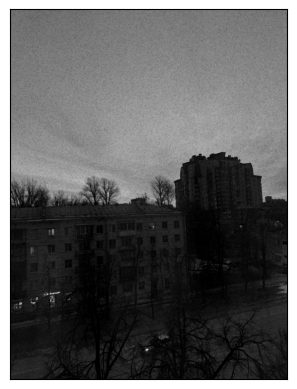
\includegraphics[width=\textwidth]{results/nlf_pois_3.png}
        \caption{Шум квантования с применением рангового фильтра}
    \end{minipage}
\end{figure}
А теперь на изображениях с максимальным параметром:
\begin{figure}[H]
    \begin{minipage}{0.49\textwidth}
        \centering 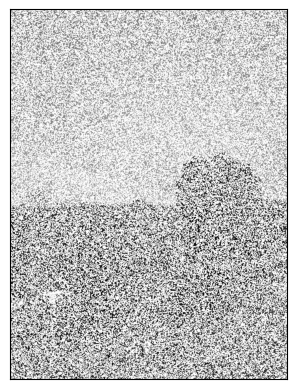
\includegraphics[width=\textwidth]{results/nlf_sap_4.png}
        \caption{Импульсный шум с применением рангового фильтра}
    \end{minipage}\hfill
    \begin{minipage}{0.49\textwidth}
        \centering 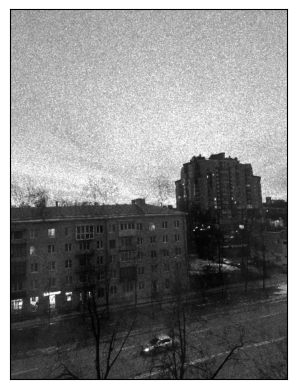
\includegraphics[width=\textwidth]{results/nlf_speckle_4.png}
        \caption{Мультипликативный шум с применением рангового фильтра}
    \end{minipage}
\end{figure}
\begin{figure}[H]
    \begin{minipage}{0.49\textwidth}
        \centering 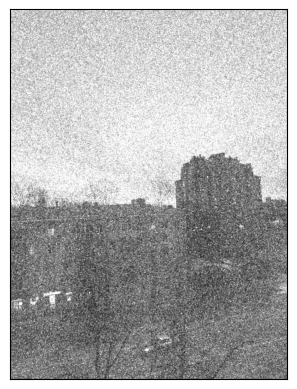
\includegraphics[width=\textwidth]{results/nlf_gaus_4.png}
        \caption{Гауссов шум с применением рангового фильтра}
    \end{minipage}\hfill
    \begin{minipage}{0.49\textwidth}
        \centering 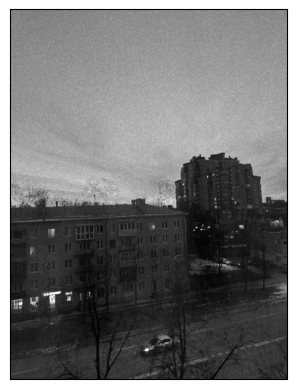
\includegraphics[width=\textwidth]{results/nlf_pois_4.png}
        \caption{Шум квантования с применением рангового фильтра}
    \end{minipage}
\end{figure}
\subsection{Винеровская фильтрация}
Винеровская (Wiener) фильтрация в общем случае не является чисто «ранговой», но часто рассматривается как нелинейная обработка при априорном учёте статистических свойств шума и сигнала. Она основана на минимизации среднеквадратической ошибки между восстановленным изображением и исходным:
\[
I_{\text{out}} = \mathcal{F}^{-1}\!\Bigl\{\, 
  \frac{H^*(\omega)}{\lvert H(\omega)\rvert^2 + S_n(\omega)/S_i(\omega)}
  \cdot G(\omega)
\Bigr\},
\]
где \(H(\omega)\) --- передаточная функция размыва, \(G(\omega)\) --- Фурье-образ зашумлённого изображения, \(S_n(\omega)\) и \(S_i(\omega)\) --- спектральные плотности шума и исходного изображения соответственно. В пространственной области реализуется адаптивная стратегия, учитывающая локальную дисперсию шума и сигнала. 
\begin{figure}[H]
    \begin{minipage}{0.49\textwidth}
        \centering 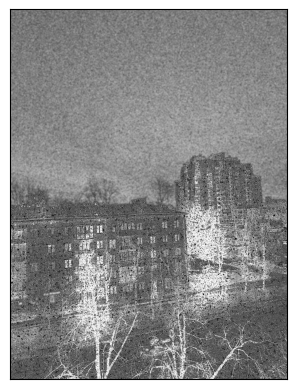
\includegraphics[width=\textwidth]{results/nlf_sap_6.png}
        \caption{Импульсный шум с применением винеровского фильтра}
    \end{minipage}\hfill
    \begin{minipage}{0.49\textwidth}
        \centering \includegraphics[width=\textwidth]{results/nlf_speckle_6.png}
        \caption{Мультипликативный шум с применением винеровского фильтра}
    \end{minipage}
\end{figure}
\begin{figure}[H]
    \begin{minipage}{0.49\textwidth}
        \centering \includegraphics[width=\textwidth]{results/nlf_gaus_6.png}
        \caption{Гауссов шум с применением винеровского фильтра}
    \end{minipage}\hfill
    \begin{minipage}{0.49\textwidth}
        \centering \includegraphics[width=\textwidth]{results/nlf_pois_6.png}
        \caption{Шум квантования с применением винеровского фильтра}
    \end{minipage}
\end{figure}
\noindent
В итоге Винеровский фильтр эффективно подавляет мультипликативный шум, но при сильных выбросах (импульсном шуме) может быть менее эффективен по сравнению с медианными методами.
\section{Высокочастотная фильтрация}
Высокочастотные фильтры позволяют выделить резкие изменения яркости (границы объектов, детали текстуры) и часто применяются для решения задач распознавания и анализа изображений. Ниже приведены основные методы выделения контуров.

\subsection{Фильтр Робертса}
Фильтр Робертса (Roberts Cross) --- один из самых простых операторов градиентного типа. Он использует два небольших \(2\times 2\) ядра:
\[
G_x = 
\begin{bmatrix}
+1 & 0 \\
0 & -1 
\end{bmatrix},
\quad
G_y =
\begin{bmatrix}
0 & +1 \\
-1 & 0 
\end{bmatrix}.
\]
После свёртки изображения с каждым ядром величина градиента вычисляется как:
\[
G = \sqrt{G_x^2 + G_y^2}.
\]
Фильтр Робертса чувствителен к шумам, так как оперирует очень малым окном, но зато даёт тонкие контуры.
\begin{figure}[H]
    \centering \includegraphics[width=0.7\textwidth]{results/hpf_1.png}
    \caption{Исходное изображение с применением фильтра Робертса}
\end{figure}
\subsection{Фильтр Превитта}
Фильтр Превитта (Prewitt Filter) использует чуть более «широкие» маски:
\[
P_x = 
\begin{bmatrix}
-1 & 0 & +1 \\
-1 & 0 & +1 \\
-1 & 0 & +1 
\end{bmatrix},
\quad
P_y =
\begin{bmatrix}
-1 & -1 & -1 \\
0 &  0 &  0 \\
+1 & +1 & +1 
\end{bmatrix}.
\]
Аналогично Робертсу, сначала вычисляются свёртки с \(P_x\) и \(P_y\), затем формируется итоговая карта градиента:
\[
G = \sqrt{G_x^2 + G_y^2}.
\]
По сравнению с оператором Робертса, фильтр Превитта даёт более стабильные результаты и менее чувствителен к шуму благодаря большему окну свёртки.
\begin{figure}[H]
    \centering \includegraphics[width=0.7\textwidth]{results/hpf_2.png}
    \caption{Исходное изображение с применением фильтра Превитта}
\end{figure}
\subsection{Фильтр Собела}
Фильтр Собела (Sobel Filter) --- наиболее часто используемый оператор для выделения контуров. Его ядра имеют дополнительный вес в центральном ряду/столбце, что повышает стабильность вычислений:
\[
S_x = 
\begin{bmatrix}
-1 & 0 & +1 \\
-2 & 0 & +2 \\
-1 & 0 & +1 
\end{bmatrix},
\quad
S_y =
\begin{bmatrix}
-1 & -2 & -1 \\
0 &  0 &  0 \\
+1 & +2 & +1 
\end{bmatrix}.
\]
Величина градиента:
\[
G = \sqrt{G_x^2 + G_y^2},
\]
где \(G_x\) и \(G_y\) --- результат свёртки исходного изображения с \(S_x\) и \(S_y\) соответственно. Фильтр Собела хорошо подавляет шумы по сравнению с более простыми операторами (Робертса, Превитта), но всё ещё уязвим к крупным выбросам.
\begin{figure}[H]
    \centering \includegraphics[width=0.7\textwidth]{results/hpf_3.png}
    \caption{Исходное изображение с применением фильтра Превитта}
\end{figure}
\subsection{Фильтр Лапласа}
Фильтр Лапласа (Laplace Filter) --- это оператор второго порядка, вычисляющий вторую производную:
\[
\nabla^2 I(x,y) \;=\; \frac{\partial^2 I}{\partial x^2} \;+\; \frac{\partial^2 I}{\partial y^2}.
\]
В дискретном виде часто используется \(3 \times 3\) ядро:
\[
L = 
\begin{bmatrix}
0 & +1 & 0 \\
+1 & -4 & +1 \\
0 & +1 & 0
\end{bmatrix},
\quad
\text{или}
\quad
\begin{bmatrix}
+1 & +1 & +1 \\
+1 & -8 & +1 \\
+1 & +1 & +1
\end{bmatrix}.
\]
Результат фильтра Лапласа обычно берут по модулю (\(\lvert \nabla^2 I\rvert\)), так как значения могут быть положительными или отрицательными. Данный оператор выделяет границы в тех местах, где функция яркости имеет значительный перегиб.
\begin{figure}[H]
    \centering \includegraphics[width=0.7\textwidth]{results/hpf_3.png}
    \caption{Исходное изображение с применением фильтра Лапласа}
\end{figure}
\subsection{Алгоритм Кэнни}
Алгоритм Кэнни (Canny Edge Detector) --- многоэтапный метод выделения контуров, включающий:
\begin{enumerate}
    \item Сглаживание изображения для подавления высокочастотных шумов.
    \item Вычисление градиентов (например, оператором Собела).
    \item Нелокальное подавление немаксимумов (Non-Maximum Suppression) для тонкого выделения линий контуров.
    \item Двойная пороговая фильтрация и отслеживание контуров (Hysteresis Thresholding): пиксели выше верхнего порога считаются надёжными границами, а пиксели между нижним и верхним порогом помечаются как границы, если они связаны с уже «надёжными» пикселями.
\end{enumerate}
Алгоритм Кэнни считается одним из самых точных методов для выделения контуров, так как сочетает в себе сглаживание шума, точное определение границ и умный механизм двойной пороговой фильтрации.
\begin{figure}[H]
    \centering \includegraphics[width=0.7\textwidth]{results/hpf_4.png}
    \caption{Исходное изображение с применением фильтра Кэнни}
\end{figure}

\section{Вопросы к защите}
\begin{enumerate}
    \item \textbf{В чём заключаются основные недостатки адаптивных методов фильтрации изображений?}\\[0.3em]
    Основной недостаток адаптивных фильтров --- возросшее время вычислений, поскольку параметры фильтра меняются «на лету» при обработке каждого пикселя. Если требуется высокая производительность, может оказаться целесообразным использовать более быстрые, неадаптивные методы фильтрации.

    \item \textbf{При каких значениях параметра \(Q\) контргармонический фильтр работает как арифметический, а при каких --- как гармонический?}\\[0.3em]
    Контргармонический фильтр эквивалентен арифметическому при \(Q = 0\) и гармоническому при \(Q = -1\).

    \item \textbf{Какими операторами можно выделить границы на изображении?}\\[0.3em]
    Для выделения границ используются дифференциальные операторы Робертса, Превитта, Собела, а также оператор Лапласа. Дополнительно можно применять многоэтапный алгоритм Кэнни.

    \item \textbf{Для чего на первом шаге выделения контуров, как правило, выполняется низкочастотная фильтрация?}\\[0.3em]
    Низкочастотная фильтрация помогает подавить мелкие шумы и незначительные детали, чтобы при последующем выделении контуров не возникало ложных границ. Это позволяет сконцентрироваться на более существенных изменениях яркости.
\end{enumerate}


\end{document}
